\documentclass{standalone}
\usepackage{tikz}
\usetikzlibrary{patterns, positioning}


\begin{document}
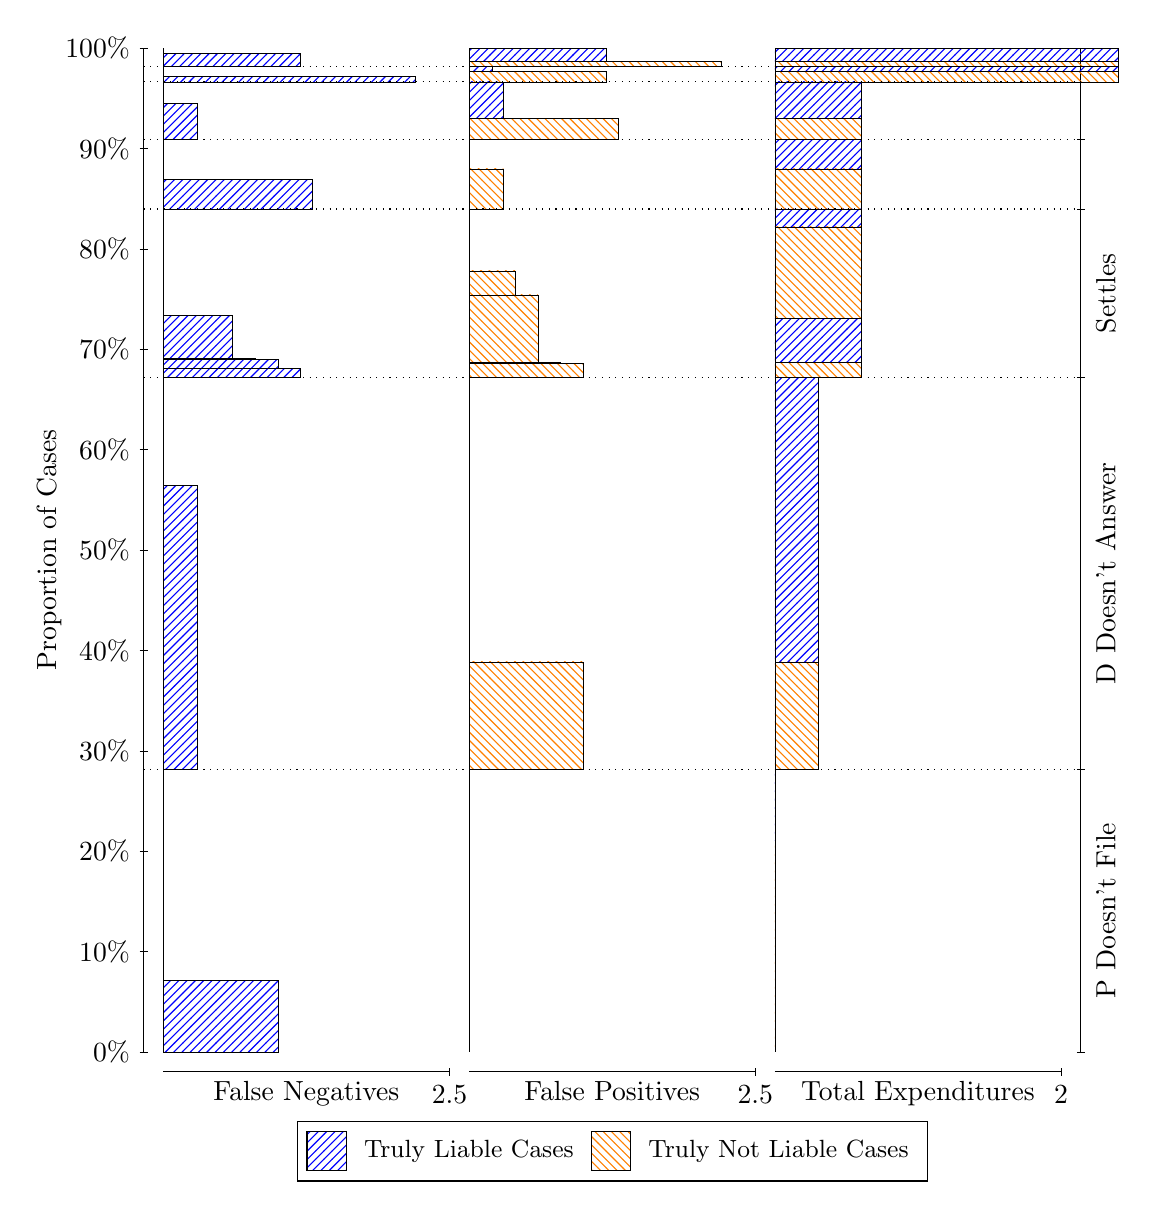
\begin{tikzpicture}
\draw[black, very thin] (1.5,1.75) -- (1.5,14.5);
\node[rotate=90, text=black, anchor=center] at (0.3, 8.125) {Proportion of Cases};
\draw[black, very thin] (1.45,1.75) -- (1.55,1.75);
\node[text=black, anchor=east] at (1.45, 1.75) {0\%};
\draw[black, very thin] (1.45,3.025) -- (1.55,3.025);
\node[text=black, anchor=east] at (1.45, 3.025) {10\%};
\draw[black, very thin] (1.45,4.3) -- (1.55,4.3);
\node[text=black, anchor=east] at (1.45, 4.3) {20\%};
\draw[black, very thin] (1.45,5.575) -- (1.55,5.575);
\node[text=black, anchor=east] at (1.45, 5.575) {30\%};
\draw[black, very thin] (1.45,6.85) -- (1.55,6.85);
\node[text=black, anchor=east] at (1.45, 6.85) {40\%};
\draw[black, very thin] (1.45,8.125) -- (1.55,8.125);
\node[text=black, anchor=east] at (1.45, 8.125) {50\%};
\draw[black, very thin] (1.45,9.4) -- (1.55,9.4);
\node[text=black, anchor=east] at (1.45, 9.4) {60\%};
\draw[black, very thin] (1.45,10.675) -- (1.55,10.675);
\node[text=black, anchor=east] at (1.45, 10.675) {70\%};
\draw[black, very thin] (1.45,11.95) -- (1.55,11.95);
\node[text=black, anchor=east] at (1.45, 11.95) {80\%};
\draw[black, very thin] (1.45,13.225) -- (1.55,13.225);
\node[text=black, anchor=east] at (1.45, 13.225) {90\%};
\draw[black, very thin] (1.45,14.5) -- (1.55,14.5);
\node[text=black, anchor=east] at (1.45, 14.5) {100\%};

\draw[black, very thin] (13.4,1.75) -- (13.4,14.5);
\draw[black, very thin] (13.35,1.75) -- (13.45,1.75);
\node[anchor=west] at (13.35, 1.75) {};
\draw[black, very thin] (13.35,5.3405) -- (13.45,5.3405);
\node[anchor=west] at (13.35, 5.3405) {};
\draw[black, very thin] (13.35,10.314) -- (13.45,10.314);
\node[anchor=west] at (13.35, 10.314) {};
\draw[black, very thin] (13.35,12.456) -- (13.45,12.456);
\node[anchor=west] at (13.35, 12.456) {};
\draw[black, very thin] (13.35,13.34) -- (13.45,13.34);
\node[anchor=west] at (13.35, 13.34) {};
\draw[black, very thin] (13.35,14.071) -- (13.45,14.071);
\node[anchor=west] at (13.35, 14.071) {};
\draw[black, very thin] (13.35,14.265) -- (13.45,14.265);
\node[anchor=west] at (13.35, 14.265) {};
\draw[black, very thin] (13.35,14.5) -- (13.45,14.5);
\node[anchor=west] at (13.35, 14.5) {};

\draw[black, very thin, pattern color=blue, pattern=north east lines] (1.75,1.75) rectangle (3.2033,2.6602);
\draw[black, very thin, pattern color=orange, pattern=north west lines] (1.75,2.6602) rectangle (1.75,5.3405);
\draw[black, very thin, pattern color=blue, pattern=north east lines] (1.75,5.3405) rectangle (2.186,8.9494);
\draw[black, very thin, pattern color=orange, pattern=north west lines] (1.75,8.9494) rectangle (1.75,10.314);
\draw[black, very thin, pattern color=blue, pattern=north east lines] (1.75,10.314) rectangle (3.494,10.432);
\draw[black, very thin, pattern color=blue, pattern=north east lines] (1.75,10.432) rectangle (3.2033,10.541);
\draw[black, very thin, pattern color=blue, pattern=north east lines] (1.75,10.541) rectangle (2.9127,10.554);
\draw[black, very thin, pattern color=blue, pattern=north east lines] (1.75,10.554) rectangle (2.622,11.1);
\draw[black, very thin, pattern color=orange, pattern=north west lines] (1.75,11.1) rectangle (1.75,12.456);
\draw[black, very thin, pattern color=blue, pattern=north east lines] (1.75,12.456) rectangle (3.6393,12.83);
\draw[black, very thin, pattern color=orange, pattern=north west lines] (1.75,12.83) rectangle (1.75,13.34);
\draw[black, very thin, pattern color=blue, pattern=north east lines] (1.75,13.34) rectangle (2.186,13.801);
\draw[black, very thin, pattern color=orange, pattern=north west lines] (1.75,13.801) rectangle (1.75,14.071);
\draw[black, very thin, pattern color=blue, pattern=north east lines] (1.75,14.071) rectangle (4.9473,14.135);
\draw[black, very thin, pattern color=orange, pattern=north west lines] (1.75,14.135) rectangle (1.75,14.265);
\draw[black, very thin, pattern color=blue, pattern=north east lines] (1.75,14.265) rectangle (3.494,14.435);
\draw[black, very thin, pattern color=orange, pattern=north west lines] (1.75,14.435) rectangle (1.75,14.5);
\draw[black, very thin, pattern color=orange, pattern=north west lines] (5.6333,1.75) rectangle (5.6333,4.4304);
\draw[black, very thin, pattern color=blue, pattern=north east lines] (5.6333,4.4304) rectangle (5.6333,5.3405);
\draw[black, very thin, pattern color=orange, pattern=north west lines] (5.6333,5.3405) rectangle (7.0867,6.7049);
\draw[black, very thin, pattern color=blue, pattern=north east lines] (5.6333,6.7049) rectangle (5.6333,10.314);
\draw[black, very thin, pattern color=orange, pattern=north west lines] (5.6333,10.314) rectangle (7.0867,10.497);
\draw[black, very thin, pattern color=orange, pattern=north west lines] (5.6333,10.497) rectangle (6.796,10.509);
\draw[black, very thin, pattern color=orange, pattern=north west lines] (5.6333,10.509) rectangle (6.5053,11.366);
\draw[black, very thin, pattern color=orange, pattern=north west lines] (5.6333,11.366) rectangle (6.2147,11.67);
\draw[black, very thin, pattern color=blue, pattern=north east lines] (5.6333,11.67) rectangle (5.6333,12.456);
\draw[black, very thin, pattern color=orange, pattern=north west lines] (5.6333,12.456) rectangle (6.0693,12.966);
\draw[black, very thin, pattern color=blue, pattern=north east lines] (5.6333,12.966) rectangle (5.6333,13.34);
\draw[black, very thin, pattern color=orange, pattern=north west lines] (5.6333,13.34) rectangle (7.5227,13.61);
\draw[black, very thin, pattern color=blue, pattern=north east lines] (5.6333,13.61) rectangle (6.0693,14.071);
\draw[black, very thin, pattern color=orange, pattern=north west lines] (5.6333,14.071) rectangle (7.3773,14.2);
\draw[black, very thin, pattern color=blue, pattern=north east lines] (5.6333,14.2) rectangle (5.924,14.265);
\draw[black, very thin, pattern color=orange, pattern=north west lines] (5.6333,14.265) rectangle (8.8307,14.33);
\draw[black, very thin, pattern color=blue, pattern=north east lines] (5.6333,14.33) rectangle (7.3773,14.5);
\draw[black, very thin, pattern color=orange, pattern=north west lines] (9.5167,1.75) rectangle (9.5167,4.4304);
\draw[black, very thin, pattern color=blue, pattern=north east lines] (9.5167,4.4304) rectangle (9.5167,5.3405);
\draw[black, very thin, pattern color=orange, pattern=north west lines] (9.5167,5.3405) rectangle (10.062,6.7049);
\draw[black, very thin, pattern color=blue, pattern=north east lines] (9.5167,6.7049) rectangle (10.062,10.314);
\draw[black, very thin, pattern color=orange, pattern=north west lines] (9.5167,10.314) rectangle (10.607,10.509);
\draw[black, very thin, pattern color=blue, pattern=north east lines] (9.5167,10.509) rectangle (10.607,11.068);
\draw[black, very thin, pattern color=orange, pattern=north west lines] (9.5167,11.068) rectangle (10.607,12.229);
\draw[black, very thin, pattern color=blue, pattern=north east lines] (9.5167,12.229) rectangle (10.607,12.456);
\draw[black, very thin, pattern color=orange, pattern=north west lines] (9.5167,12.456) rectangle (10.607,12.966);
\draw[black, very thin, pattern color=blue, pattern=north east lines] (9.5167,12.966) rectangle (10.607,13.34);
\draw[black, very thin, pattern color=orange, pattern=north west lines] (9.5167,13.34) rectangle (10.607,13.61);
\draw[black, very thin, pattern color=blue, pattern=north east lines] (9.5167,13.61) rectangle (10.607,14.071);
\draw[black, very thin, pattern color=orange, pattern=north west lines] (9.5167,14.071) rectangle (13.877,14.2);
\draw[black, very thin, pattern color=blue, pattern=north east lines] (9.5167,14.2) rectangle (13.877,14.265);
\draw[black, very thin, pattern color=orange, pattern=north west lines] (9.5167,14.265) rectangle (13.877,14.33);
\draw[black, very thin, pattern color=blue, pattern=north east lines] (9.5167,14.33) rectangle (13.877,14.5);
\draw[black, dotted] (1.5,5.3405) -- (13.4,5.3405);
\draw[black, dotted] (1.5,10.314) -- (13.4,10.314);
\draw[black, dotted] (1.5,12.456) -- (13.4,12.456);
\draw[black, dotted] (1.5,13.34) -- (13.4,13.34);
\draw[black, dotted] (1.5,14.071) -- (13.4,14.071);
\draw[black, dotted] (1.5,14.265) -- (13.4,14.265);
\draw[black, very thin] (1.75,1.5) -- (5.3833,1.5);
\node[text=black, anchor=north] at (3.5667, 1.5) {False Negatives};
\draw[black, very thin] (5.3833,1.45) -- (5.3833,1.55);
\node[text=black, anchor=north] at (5.3833, 1.45) {2.5};

\draw[black, very thin] (5.6333,1.5) -- (9.2667,1.5);
\node[text=black, anchor=north] at (7.45, 1.5) {False Positives};
\draw[black, very thin] (9.2667,1.45) -- (9.2667,1.55);
\node[text=black, anchor=north] at (9.2667, 1.45) {2.5};

\draw[black, very thin] (9.5167,1.5) -- (13.15,1.5);
\node[text=black, anchor=north] at (11.333, 1.5) {Total Expenditures};
\draw[black, very thin] (13.15,1.45) -- (13.15,1.55);
\node[text=black, anchor=north] at (13.15, 1.45) {2};

\node[text=black, centered, rotate=90] at (13.72, 3.5453) {P Doesn't File};
\node[text=black, centered, rotate=90] at (13.72, 7.8272) {D Doesn't Answer};
\node[text=black, centered, rotate=90] at (13.72, 11.385) {Settles};





\draw (7.449999999999999,1.5) node[draw=none] (baseCoordinate) {};
\begin{scope}[align=center]
        \matrix[scale=0.5, draw=black, below=0.5cm of baseCoordinate, nodes={draw}, column sep=0.1cm]{
            \node[rectangle, draw, minimum width=0.5cm, minimum height=0.5cm, pattern color=blue, pattern=north east lines] {}; &
            \node[draw=none, font=\small, text=black] (B) {Truly Liable Cases}; &
            \node[rectangle, draw, minimum width=0.5cm, minimum height=0.5cm, pattern color=orange, pattern=north west lines] {}; &
            \node[draw=none, font=\small, text=black] (B) {Truly Not Liable Cases}; \\
            };
\end{scope}

\end{tikzpicture}
\end{document}